\documentclass[tikz]{standalone}
\usepackage[utf8]{inputenc}

\definecolor{DarkRed}{rgb}{0.7,0.2,0.2}

\begin{document}

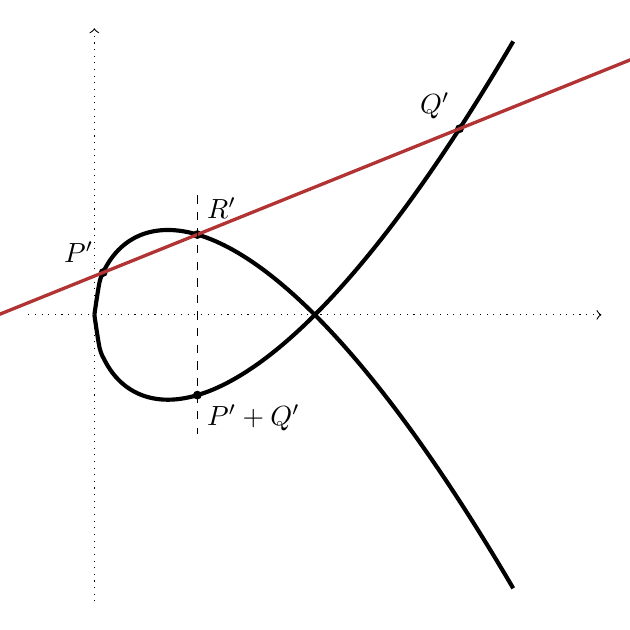
\begin{tikzpicture}[scale=2.8]
\def\ptsize{.02}
\draw[->,dotted] (-.3, 0) -- (2.3,0);
\draw[->,dotted] (0,-1.3) -- (0,1.3);
\draw[domain=0:1.9,smooth,samples=80,line width=1.5pt] plot (\x, {sqrt(\x)*(\x - 1)});
\draw[domain=0:1.9,smooth,samples=80,line width=1.5pt] plot (\x, {-sqrt(\x)*(\x - 1)});

\coordinate[label=above left:$P'$] (P) at (.04,.192);
\coordinate[label=above left:$Q'$] (Q) at (1.656,.844);
\coordinate (R) at (.467,.364);
\node[above right,shift={(0,.08)}] at (R) {$R'$};
\coordinate[label=below right:$P'+Q'$] (S) at (.467,-.364);

\fill (P) circle (\ptsize);
\fill (Q) circle (\ptsize);
\fill (R) circle (\ptsize);
\fill (S) circle (\ptsize);

\draw[DarkRed,shorten >=-3cm,shorten <=-3cm,line width=1.2pt] (P) -- (Q);
\draw[dashed,shorten >=-.5cm,shorten <=-.5cm] (R) -- (S);

\end{tikzpicture}

\end{document}